%--------------------------------------------------------------------------------------
% Dokumentum formátuma [Document format]
%--------------------------------------------------------------------------------------

%TODO Válaszd ki, hogy egyoldalas vagy kétoldalas legyen! [Choose format]
%\documentclass[12pt,a4paper,oneside]{report}             % Egyoldalas [Single-side]
\documentclass[12pt,a4paper,twoside,openright]{report}  % Kétoldalas [Duplex]


%--------------------------------------------------------------------------------------
% Csomagok inicializálása [Initializing packages]
%--------------------------------------------------------------------------------------
\usepackage{ifthen} % Used in macros

\usepackage[english,magyar]{babel} % Language support
\usepackage{geometry}
\usepackage{amsfonts,amsmath,amssymb} % Mathematical symbols
\usepackage{microtype} % Imrovements to typesetting
\usepackage{setspace} % For setting line spacing
\usepackage{cmap} % Enables more advenced text copying from the PDF document 
\usepackage{sectsty} % Section heading styling

\usepackage[unicode]{hyperref} % For hyperlinks in the generated document
\usepackage{booktabs} % For publication quality tables for LaTeX
\usepackage{graphicx} % For figure sizing
\usepackage[hang]{caption}
\usepackage{xcolor} % For code coloring in listings
\usepackage{listings} % For source code snippets
\usepackage[amsmath,thmmarks]{ntheorem} % Theorem-like environments

\usepackage[numbers]{natbib} % Bibliography

\usepackage{enumerate}% Roman numerals in enumerate
\usepackage{hhline}% Double line in tables
\usepackage{gensymb}% Symbols
\usepackage{icomma}% Hungarian comma in equations

%\usepackage{fancyhdr} % For easy to use headers and footers

% thanks to http://tex.stackexchange.com/a/47579/71109
\usepackage{ifxetex}
\usepackage{ifluatex}
\newif\ifxetexorluatex % a new conditional starts as false
\ifnum 0\ifxetex 1\fi\ifluatex 1\fi>0
   \xetexorluatextrue
\fi

\ifxetexorluatex
  \usepackage{fontspec}
  % Palatino clone font (Tex Gyre Pagella) for text and math
  \usepackage{newpxmath}
  \setmainfont[Ligatures=TeX]{TeX Gyre Pagella}
\else
  \usepackage[T1]{fontenc}
  \usepackage[utf8]{inputenc}
  %\usepackage[lighttt]{lmodern} % Advanced version of the Computer Modern font
  % Palatino clone font (Tex Gyre Pagella) for text and math
  \usepackage{tgpagella, newpxmath}
\fi



%--------------------------------------------------------------------------------------
% Dokumentum nyelve [Language]
%--------------------------------------------------------------------------------------

%TODO Válaszd ki a nyelvet! [Select language]
%--------------------------------------------------------------------------------------
% Elnevezések
%--------------------------------------------------------------------------------------
\newcommand{\bme}{Budapesti Műszaki és Gazdaságtudományi Egyetem}
\newcommand{\gpk}{Gépészmérnöki Kar}

\newcommand{\bmeatt}{Anyagtudomány és Technológia Tanszék}
\newcommand{\bmeara}{Áramlástan Tanszék}
\newcommand{\bmeenergia}{Energetikai Gépek és Rendszerek Tanszék}
\newcommand{\bmeepget}{Épületgépészeti és Gépészeti Eljárástechnika Tanszék}
\newcommand{\bmegtharom}{Gép- és Terméktervezés Tanszék}
\newcommand{\bmemanuf}{Gyártástudomány és -technológia Tanszék}
\newcommand{\bmehds}{Hidrodinamikai Rendszerek Tanszék}
\newcommand{\bmemogi}{Mechatronika, Optika és Gépészeti Informatika Tanszék}
\newcommand{\bmemm}{Műszaki Mechanika Tanszék}
\newcommand{\bmept}{Polimertechnika Tanszék}

\newcommand{\keszitette}{Készítette}
\newcommand{\konzulens}{Konzulens}
\newcommand{\temavezeto}{Témavezető}

\newcommand{\selectbsc}{
  \newcommand{\gpkmunkatipus}{Szakdolgozat}       % Dokumentum típusa [Document type]
  \newcommand{\gpkmunkatipusHU}{Szakdolgozat}     % Dokumentum típusa HU
  \newcommand{\gpkmunkatipusok}{Szakdolgozatok}   % többesszámban
  \newcommand{\gpkmunkatipustHU}{Szakdolgozatot}  % tárgyraggal
}
\newcommand{\selectmsc}{
  \newcommand{\gpkmunkatipus}{Diplomaterv}        % Dokumentum típusa [Document type]
  \newcommand{\gpkmunkatipusHU}{Diplomaterv}      % Dokumentum típusa HU
  \newcommand{\gpkmunkatipusok}{Diplomatervek}    % többesszámban
  \newcommand{\gpkmunkatipustHU}{Diplomatervet}   % tárgyraggal
}

\newcommand{\tdk}{TDK dolgozat}
\newcommand{\bsconlab}{BSc Önálló laboratórium}
\newcommand{\msconlabi}{MSc Önálló laboratórium 1.}
\newcommand{\msconlabii}{MSc Önálló laboratórium 2.}

\newcommand{\szerzoijog}{Szerzői jog}

\newcommand{\pelda}{Példa}
\newcommand{\definicio}{Definíció}
\newcommand{\tetel}{Tétel}

\newcommand{\jelolesek}{Jelölések jegyzéke}
\newcommand{\eloszo}{Előszó}
\newcommand{\bevezetes}{Bevezetés}
\newcommand{\koszonetnyilvanitas}{Köszönetnyilvánítás}
\newcommand{\osszefoglalas}{Összefoglalás}
\newcommand{\summary}{Summary}
\newcommand{\fuggelek}{Függelék}
\newcommand{\melleklet}{Mellékletek}

% Opcionálisan átnevezhető címek
\addto\captionsmagyar{%
\renewcommand{\listfigurename}{Illusztrációk jegyzéke}
%\renewcommand{\listtablename}{Saját táblázatjegyzék cím}
%\renewcommand{\bibname}{Saját irodalomjegyzék név}
}

\newcommand{\authorName}{\authorFamilyName{} \authorGivenName}
\newcommand{\consulentA}{\consulentATitle\consulentAFamilyName{} \consulentAGivenName}
\newcommand{\consulentB}{\consulentBTitle\consulentBFamilyName{} \consulentBGivenName}
\newcommand{\consulentC}{\consulentCTitle\consulentCFamilyName{} \consulentCGivenName}
\newcommand{\supervisor}{\supervisorTitle\supervisorFamilyName{}
\supervisorGivenName}

\newcommand{\selectthesislanguage}{\selecthungarian}
\newcommand{\selectforeignlanguage}{\selectenglish}

\bibliographystyle{huplain}

\def\lstlistingname{lista}

\newcommand{\appendixletter}{6} % a fofejezet-szamlalo az angol ABC 6. betuje (F) lesz
\newcommand{\annexletter}{13} % M betű
 % Beállítások magyar nyelvű dolgozathoz
%%--------------------------------------------------------------------------------------
% Elnevezések
%--------------------------------------------------------------------------------------
\newcommand{\bme}{Budapest University of Technology and Economics}
\newcommand{\gpk}{Faculty of Mechanical Engineering}

\newcommand{\bmeatt}{Department of Materials Science and Engineering}
\newcommand{\bmeara}{Department of Fluid Mechanics}
\newcommand{\bmeenergia}{Department of Energy Engineering}
\newcommand{\bmeepget}{Department of Building Service Engineering and Process Engineering}
\newcommand{\bmegtharom}{Department of Machine and Product Design}
\newcommand{\bmemanuf}{Department of Manufacturing Science and Engineering}
\newcommand{\bmehds}{Department of Hydrodynamic Systems}
\newcommand{\bmemogi}{Department of Mechatornics, Optics and Mechanical Engineering Informatics}
\newcommand{\bmemm}{Department of Applied Mechanics}
\newcommand{\bmept}{Department of Polymer Engineering}

\newcommand{\keszitette}{Author}
\newcommand{\konzulens}{Advisor}
\newcommand{\temavezeto}{Supervisor}

\newcommand{\selectbsc}{
  \newcommand{\gpkmunkatipus}{Bachelor's Thesis}  % Dokumentum típusa [Document type]
  \newcommand{\gpkmunkatipusHU}{Szakdolgozat}     % Dokumentum típusa HU
  \newcommand{\gpkmunkatipusok}{Bachelor's Theses}% többesszámban
  \newcommand{\gpkmunkatipustHU}{Szakdolgozatot}  % tárgyraggal
}
\newcommand{\selectmsc}{
  \newcommand{\gpkmunkatipus}{Master's Thesis}    % Dokumentum típusa [Document type]
  \newcommand{\gpkmunkatipusHU}{Diplomaterv}      % Dokumentum típusa HU
  \newcommand{\gpkmunkatipusok}{Master's Theses}  % többesszámban
  \newcommand{\gpkmunkatipustHU}{Diplomatervet}   % tárgyraggal
}

\newcommand{\tdk}{Scientific Students' Association Report}
\newcommand{\bsconlab}{BSc Project Laboratory}
\newcommand{\msconlabi}{MSc Project Laboratory 1}
\newcommand{\msconlabii}{MSc Project Laboratory 2}

\newcommand{\szerzoijog}{Copyright}

\newcommand{\pelda}{Example}
\newcommand{\definicio}{Definition}
\newcommand{\tetel}{Theorem}

\newcommand{\jelolesek}{Symbols}
\newcommand{\eloszo}{Abstract}
\newcommand{\bevezetes}{Introduction}
\newcommand{\koszonetnyilvanitas}{Acknowledgements}
\newcommand{\osszefoglalas}{Summary}
\newcommand{\summary}{Összefoglalás}
\newcommand{\fuggelek}{Appendix}
\newcommand{\melleklet}{Annex}

\renewcommand{\figureautorefname}{Figure}
\renewcommand{\tableautorefname}{Table}
\renewcommand{\partautorefname}{Part}
\renewcommand{\chapterautorefname}{Chapter}
\renewcommand{\sectionautorefname}{Section}
\renewcommand{\subsectionautorefname}{Section}
\renewcommand{\subsubsectionautorefname}{Section}

% Optional custom titles
%\addto\captionsenglish{%
%\renewcommand*{\listfigurename}{Your list of figures title}
%\renewcommand*{\listtablename}{Your list of tables title}
%\renewcommand*{\bibname}{Your bibliography title}
%}

\newcommand{\authorName}{\authorGivenName{} \authorFamilyName}
\newcommand{\consulentA}{\consulentATitle\consulentAGivenName{} \consulentAFamilyName}
\newcommand{\consulentB}{\consulentBTitle\consulentBGivenName{} \consulentBFamilyName}
\newcommand{\consulentC}{\consulentCTitle\consulentCGivenName{} \consulentCFamilyName}
\newcommand{\supervisor}{\supervisorTitle\supervisorGivenName{} \supervisorFamilyName}

\newcommand{\selectthesislanguage}{\selectenglish}
\newcommand{\selectforeignlanguage}{\selecthungarian}

\bibliographystyle{plainnat}

\newcommand{\ie}{i.e.\@\xspace}
\newcommand{\Ie}{I.e.\@\xspace}
\newcommand{\eg}{e.g.\@\xspace}
\newcommand{\Eg}{E.g.\@\xspace}
\newcommand{\etal}{et al.\@\xspace}
\newcommand{\etc}{etc.\@\xspace}
\newcommand{\vs}{vs.\@\xspace}
\newcommand{\viz}{viz.\@\xspace} % videlicet
\newcommand{\cf}{cf.\@\xspace} % confer
\newcommand{\Cf}{Cf.\@\xspace}
\newcommand{\wrt}{w.r.t.\@\xspace} % with respect to
\newcommand{\approximately}{approx.\@\xspace}

\newcommand{\appendixletter}{1}  % a fofejezet-szamlalo az angol ABC 1. betuje (A) lesz
\newcommand{\annexletter}{2} % B betű
    % Settings for English document

% Megjegyzés: 
%         Ez a beállítás az automatikusan létrehozott címek, hivatkozások
%         nyelvét adja meg, valamint a nyelvre jellemző behúzási távolságot
%         használja a bekezdések elején.
%
% Note: 
%         This setting controls the language of generated titles and citations,
%         moreover the paragraph indentation.


%--------------------------------------------------------------------------------------
% Preambulum (LaTeX beállítások, makrók) [Preamble (LaTeX settings)]
%--------------------------------------------------------------------------------------
%--------------------------------------------------------------------------------------
% Page layout setup
%--------------------------------------------------------------------------------------
% we need to redefine the pagestyle plain
% another possibility is to use the body of this command without \fancypagestyle
% and use \pagestyle{fancy} but in that case the special pages
% (like the ToC, the References, and the Chapter pages)remain in plane style

\pagestyle{plain}
\geometry{inner=30mm, outer=20mm, top=20mm, bottom=30mm}


%--------------------------------------------------------------------------------------
% Text and paragraph styling
%--------------------------------------------------------------------------------------

\sectionfont{\Large\upshape\bfseries}  % Section title font
\subsectionfont{\Large\itshape\mdseries}
\subsubsectionfont{\large\itshape\mdseries}
\setcounter{secnumdepth}{3}             % Section numbering depth

\sloppy                                 % Prevent text from spilling over the margin
\widowpenalty=10000 \clubpenalty=10000  % Prevent widow and oprhan rows
\def\hyph{-\penalty0\hskip0pt\relax}    % Enable hyphenation

\onehalfspacing                         % 1.5x Line spacing

% Text setup for Hungarian text
\newcommand{\selecthungarian}{
	\selectlanguage{magyar}
	\setlength{\parindent}{2em}			% Paragraph indentation
	\setlength{\parskip}{5pt}			% Paragraph spacing
	\frenchspacing
}

% Text setup for English text
\newcommand{\selectenglish}{
	\selectlanguage{english}
	\setlength{\parindent}{0em}
	\setlength{\parskip}{8pt}
	\nonfrenchspacing
}

%--------------------------------------------------------------------------------------
% Setup hyperref package
%--------------------------------------------------------------------------------------
\hypersetup{
    % bookmarks=true,            % show bookmarks bar?
    unicode=true,                % non-Latin characters in Acrobat's bookmarks
    pdfnewwindow=true,           % links in new window
    colorlinks=true,             % false: boxed links; true: colored links
    linkcolor=black,             % color of internal links
    citecolor=black,             % color of links to bibliography
    filecolor=black,             % color of file links
    urlcolor=black               % color of external links
}

%--------------------------------------------------------------------------------------
% Apply variables
%--------------------------------------------------------------------------------------
% This command is called in the main tex file and uses variables set there.
\newcommand{\applyvariables}{
	\author{\authorName}
	\title{\thesisTitle}

	\hypersetup{
		pdftitle={\thesisTitle},     % title
		pdfauthor={\authorName},     % author
		pdfsubject={\gpkmunkatipus}, % subject of the document
		pdfkeywords={\keywords},     % list of keywords (separate then by comma)
		pdfproducer={\authorName},   % producer of the document (organization)
		pdfcreator={LaTeX}           % creator of the document (application)
	}
}

%--------------------------------------------------------------------------------------
% Set up listings
%--------------------------------------------------------------------------------------
\definecolor{lightgray}{rgb}{0.95,0.95,0.95}
\lstset{
	basicstyle=\scriptsize\ttfamily, % print whole listing small
	keywordstyle=\color{black}\bfseries, % bold black keywords
	identifierstyle=, % nothing happens
	% default behavior: comments in italic, to change use
	% commentstyle=\color{green}, % for e.g. green comments
	stringstyle=\scriptsize,
	showstringspaces=false, % no special string spaces
	aboveskip=3pt,
	belowskip=3pt,
	backgroundcolor=\color{lightgray},
	columns=flexible,
	keepspaces=true,
	escapeinside={(*@}{@*)},
	captionpos=b,
	breaklines=true,
	frame=single,
	float=!ht,
	tabsize=2,
	literate=*
		{á}{{\'a}}1	{é}{{\'e}}1	{í}{{\'i}}1	{ó}{{\'o}}1	{ö}{{\"o}}1	{ő}{{\H{o}}}1	{ú}{{\'u}}1	{ü}{{\"u}}1	{ű}{{\H{u}}}1
		{Á}{{\'A}}1	{É}{{\'E}}1	{Í}{{\'I}}1	{Ó}{{\'O}}1	{Ö}{{\"O}}1	{Ő}{{\H{O}}}1	{Ú}{{\'U}}1	{Ü}{{\"U}}1	{Ű}{{\H{U}}}1
}


%--------------------------------------------------------------------------------------
% Set up theorem-like environments
%--------------------------------------------------------------------------------------
% Using ntheorem package -- see http://www.math.washington.edu/tex-archive/macros/latex/contrib/ntheorem/ntheorem.pdf

\theoremstyle{plain}
\theoremseparator{.}
\newtheorem{example}{\pelda}

\theoremseparator{.}
%\theoremprework{\bigskip\hrule\medskip}
%\theorempostwork{\hrule\bigskip}
\theorembodyfont{\upshape}
\theoremsymbol{{\large \ensuremath{\centerdot}}}
\newtheorem{definition}{\definicio}

\theoremseparator{.}
%\theoremprework{\bigskip\hrule\medskip}
%\theorempostwork{\hrule\bigskip}
\newtheorem{theorem}{\tetel}


%--------------------------------------------------------------------------------------
% Some new commands and declarations
%--------------------------------------------------------------------------------------
\newcommand{\code}[1]{{\upshape\ttfamily\scriptsize\indent #1}}
\newcommand{\doi}[1]{DOI: \href{http://dx.doi.org/\detokenize{#1}}{\raggedright{\texttt{\detokenize{#1}}}}} % A hivatkozások közt így könnyebb DOI-t megadni.

\DeclareMathOperator*{\argmax}{arg\,max}
%\DeclareMathOperator*[1]{\floor}{arg\,max}
\DeclareMathOperator{\sign}{sgn}
\DeclareMathOperator{\rot}{rot}


%--------------------------------------------------------------------------------------
% Setup captions
%--------------------------------------------------------------------------------------
\captionsetup[figure]{
	width=.75\textwidth,
	aboveskip=10pt}

\renewcommand{\captionlabelfont}{\it}
\renewcommand{\captionfont}{\footnotesize\it}

%--------------------------------------------------------------------------------------
% Hyphenation exceptions
%--------------------------------------------------------------------------------------
\hyphenation{Shakes-peare Mar-seilles ár-víz-tű-rő tü-kör-fú-ró-gép}


%--------------------------------------------------------------------------------------
% Command to exclude tables and images in the annex from the List of Figures/Tables
%--------------------------------------------------------------------------------------
\newcommand{\excludeFromLocAndLot}{
	% Redefine \addcontentsline to be silent when printing loc or toc entries
	\let\svaddcontentsline\addcontentsline
	\renewcommand\addcontentsline[3]{
		\ifthenelse{\equal{##1}{lof}}{}{
			\ifthenelse{\equal{##1}{lot}}{}{
				\svaddcontentsline{##1}{##2}{##3}
			}
		}
	}
}

%--------------------------------------------------------------------------------------
% PDF oldal beillesztéshez
%--------------------------------------------------------------------------------------
\usepackage{pdfpages}



%--------------------------------------------------------------------------------------
% Munkatípus [Thesis type]
%--------------------------------------------------------------------------------------

%TODO Válaszd ki a munkatípust [Select thesis type]
\selectbsc    % Szakdolgozat [Bachelor's]
%\selectmsc   % Diplomaterv [Master's]


%--------------------------------------------------------------------------------------
% Változók beállítása [Setting variables]
%--------------------------------------------------------------------------------------

%TODO Állítsd be az alábbi változókat [Set these variables]

% Szerző [Author]
\def\authorFamilyName{Kovács}
\def\authorGivenName{Hunor Ádám}
\def\neptun{P953MO}

% Konzulens 1 [Consulent 1]
\def\consulentATitle{}
\def\consulentAFamilyName{Vincze}
\def\consulentAGivenName{Bálint}
\def\consulentARank{Ügyvezető igazgató, HEVESGÉP Kft.}

% Konzulens 2 [Consulent 2], ha nincs hagyd üresen
\def\consulentBTitle{}
\def\consulentBFamilyName{Konzulens}
\def\consulentBGivenName{Kettő}
\def\consulentBRank{okl. gépészmérnök}

% Konzulens 3 [Consulent 3], ha nincs hagyd üresen 
\def\consulentCTitle{}
\def\consulentCFamilyName{}
\def\consulentCGivenName{}
\def\consulentCRank{}

% Témavezető
\def\supervisorTitle{}
\def\supervisorFamilyName{Haba}
\def\supervisorGivenName{Tamás}
\def\supervisorRank{PhD hallgató}

% Dolgozat címe [Thesis title]
\def\thesisTitle{Szálastakarmány felszedő adapter szenzortechnikai fejlesztése}

% Kulcsszavak (a PDF-be) [Keywords (to PDF)]
\def\keywords{mechatronika, szabályozástechnika, szálastakarmány, szenzor, mezőgazdaság}

% Tanszék [Department]
%TODO Válassz az alábbiak közül
% \bmeatt    \bmeara  \bmeenergia  \bmeepget  \bmegtharom 
% \bmemanuf  \bmehds  \bmemogi     \bmemm     \bmept
\def\department{\bmemogi}

%TODO Cseréld le a figures/tanszek_logo.pdf képet a tanszéked logójára!
%     [Replace figures/tanszek_logo.pdf with the logo of your department]

% Elzártan kezelendő dolgozat [Restricted access]
%TODO Töltsd ki a korlátozás lejártának dátumát! 
%     [Fill in the end date of the restriction]
\def\endOfRestrictedAccess{... év ... hónap ... nap}


% Változók beállítása a PDF fájlhoz [Apply variables for the PDF file]
\applyvariables


%--------------------------------------------------------------------------------------
% Dokumentum törzse [Document body]
%--------------------------------------------------------------------------------------

\begin{document}

\pagenumbering{gobble}
\selectthesislanguage

% Címoldal [Titlepage]
\hypersetup{pageanchor=false}

%--------------------------------------------------------------------------------------
% Szennycímoldal [Cover title page]
%--------------------------------------------------------------------------------------

\clearpage
\begin{center}
\MakeUppercase{\authorName}\\[0.1cm]
\MakeUppercase{\gpkmunkatipus}\\[0.1cm]
\end{center}
\thispagestyle{empty}

%--------------------------------------------------------------------------------------
% Sorozatcímoldal [Series title page]
%--------------------------------------------------------------------------------------
\clearpage
\begin{center}


\includegraphics[width=60mm,keepaspectratio]{figures/bme_logo.pdf}\\
\vspace{0.3cm}
\MakeUppercase{\textbf{\bme}}\\[0.1cm]
\MakeUppercase{\textmd{\gpk}}\\[0.1cm]
\MakeUppercase{\textmd{\department}}\\[0.8cm]


\includegraphics[height=40mm,keepaspectratio]{figures/tanszek_logo}\\[0.5cm]
\MakeUppercase{\gpkmunkatipusok}

\end{center}
\thispagestyle{empty}

%--------------------------------------------------------------------------------------
% Címoldal [Title page]
%--------------------------------------------------------------------------------------
\begin{titlepage}
\begin{center}

\includegraphics[width=60mm,keepaspectratio]{figures/bme_logo.pdf}\\
\vspace{0.3cm}
\MakeUppercase{\textbf{\bme}}\\[0.1cm]
\MakeUppercase{\textmd{\gpk}}\\[0.1cm]
\MakeUppercase{\textmd{\department}}

\vspace{4.0cm}
{\huge \textsc{\authorName}}\\[0.8cm]
{\huge \MakeUppercase{\gpkmunkatipus}}\\[0.8cm]
{\Large \thesisTitle}

\vspace{3.0cm}

{
	\renewcommand{\arraystretch}{0.85}
	\begin{tabular}{ll}
	 \makebox[7cm][l]{\konzulens:} & \makebox[7cm][l]{\temavezeto:} \\
	 \noalign{\smallskip}
	 \makebox[7cm][l]{\hspace{1cm}\emph{\consulentA}} & \makebox[7cm][l]{\hspace{1cm}\emph{\supervisor}} \\
	 \makebox[7cm][l]{\hspace{1cm}\consulentARank} & \makebox[7cm][l]{\hspace{1cm}\supervisorRank} \\
	 \\
	 \makebox[7cm][l]{\hspace{1cm}\emph{\consulentB}} & \\
	 \makebox[7cm][l]{\hspace{1cm}\consulentBRank} & \\
	 \\
	 \makebox[7cm][l]{\hspace{1cm}\emph{\consulentC}} & \\
	 \makebox[7cm][l]{\hspace{1cm}\consulentCRank} & \\
	 
	\end{tabular}
}

\vfill
{\Large Budapest, \the\year.}
\end{center}
\end{titlepage}
\hypersetup{pageanchor=false}
\thispagestyle{empty}
  % Szakdolgozat/Diplomaterv címlap [Thesis]


% Copytightoldal [Copyright page]
%TODO Válaszd ki a megfelelőt! [Choose one]
\selectlanguage{magyar}
\pagenumbering{gobble}
\selecthungarian
%--------------------------------------------------------------------------------------
% Copyrightoldal
%--------------------------------------------------------------------------------------
\begin{flushleft}
\szerzoijog{} {\textcopyright} \authorName, \the\year.
\end{flushleft}

\vfill
\clearpage
\thispagestyle{empty} % an empty page

\selectthesislanguage
               % Nyílt kezelésű [Open access]
%\selectlanguage{magyar}
\pagenumbering{gobble}
\selecthungarian
%--------------------------------------------------------------------------------------
% Copyrightoldal
%--------------------------------------------------------------------------------------
\begin{flushleft}
Szerzői jog {\textcopyright} \authorName, \the\year.
\end{flushleft}

\vspace{0.5cm}

\begin{center}
\textbf{ZÁRADÉK}\\
\end{center}

\vspace{0.5cm}
\noindent
Ez a \MakeLowercase{\gpkmunkatipusHU} elzártan kezelendő és őrzendő, a hozzáférése a vonatkozó szabályok szerint korlátozott, a dolgozat tartalmát csak az arra feljogosított személyek ismerhetik.

A korlátozott hozzáférés időtartamának lejártáig az arra feljogosítottakon kívül csak a korlátozást kérelmező személy vagy gazdálkodó szervezet írásos engedélyéjével rendelkező személy nyerhet betekintést a dolgozat tartalmába.

\vspace{0.3cm}

%TODO: fill out the date
A hozzáférés korlátozása és a zárt kezelés \endOfRestrictedAccess ján ér véget.

\vfill
\clearpage
\thispagestyle{empty} % an empty page

\selectthesislanguage
   % Elzárt kezelésű [Restricted access]


% Feladatkiírás [Project page]
%TODO A nyomtatott verzóban ne szerepeljen! [Remove before printing]
%--------------------------------------------------------------------------------------
% Feladatkiiras (a tanszeken atveheto, kinyomtatott valtozat)
%--------------------------------------------------------------------------------------
\thispagestyle{empty}

% a kiírási oldal helyén: feladatkiiras beillesztese
\noindent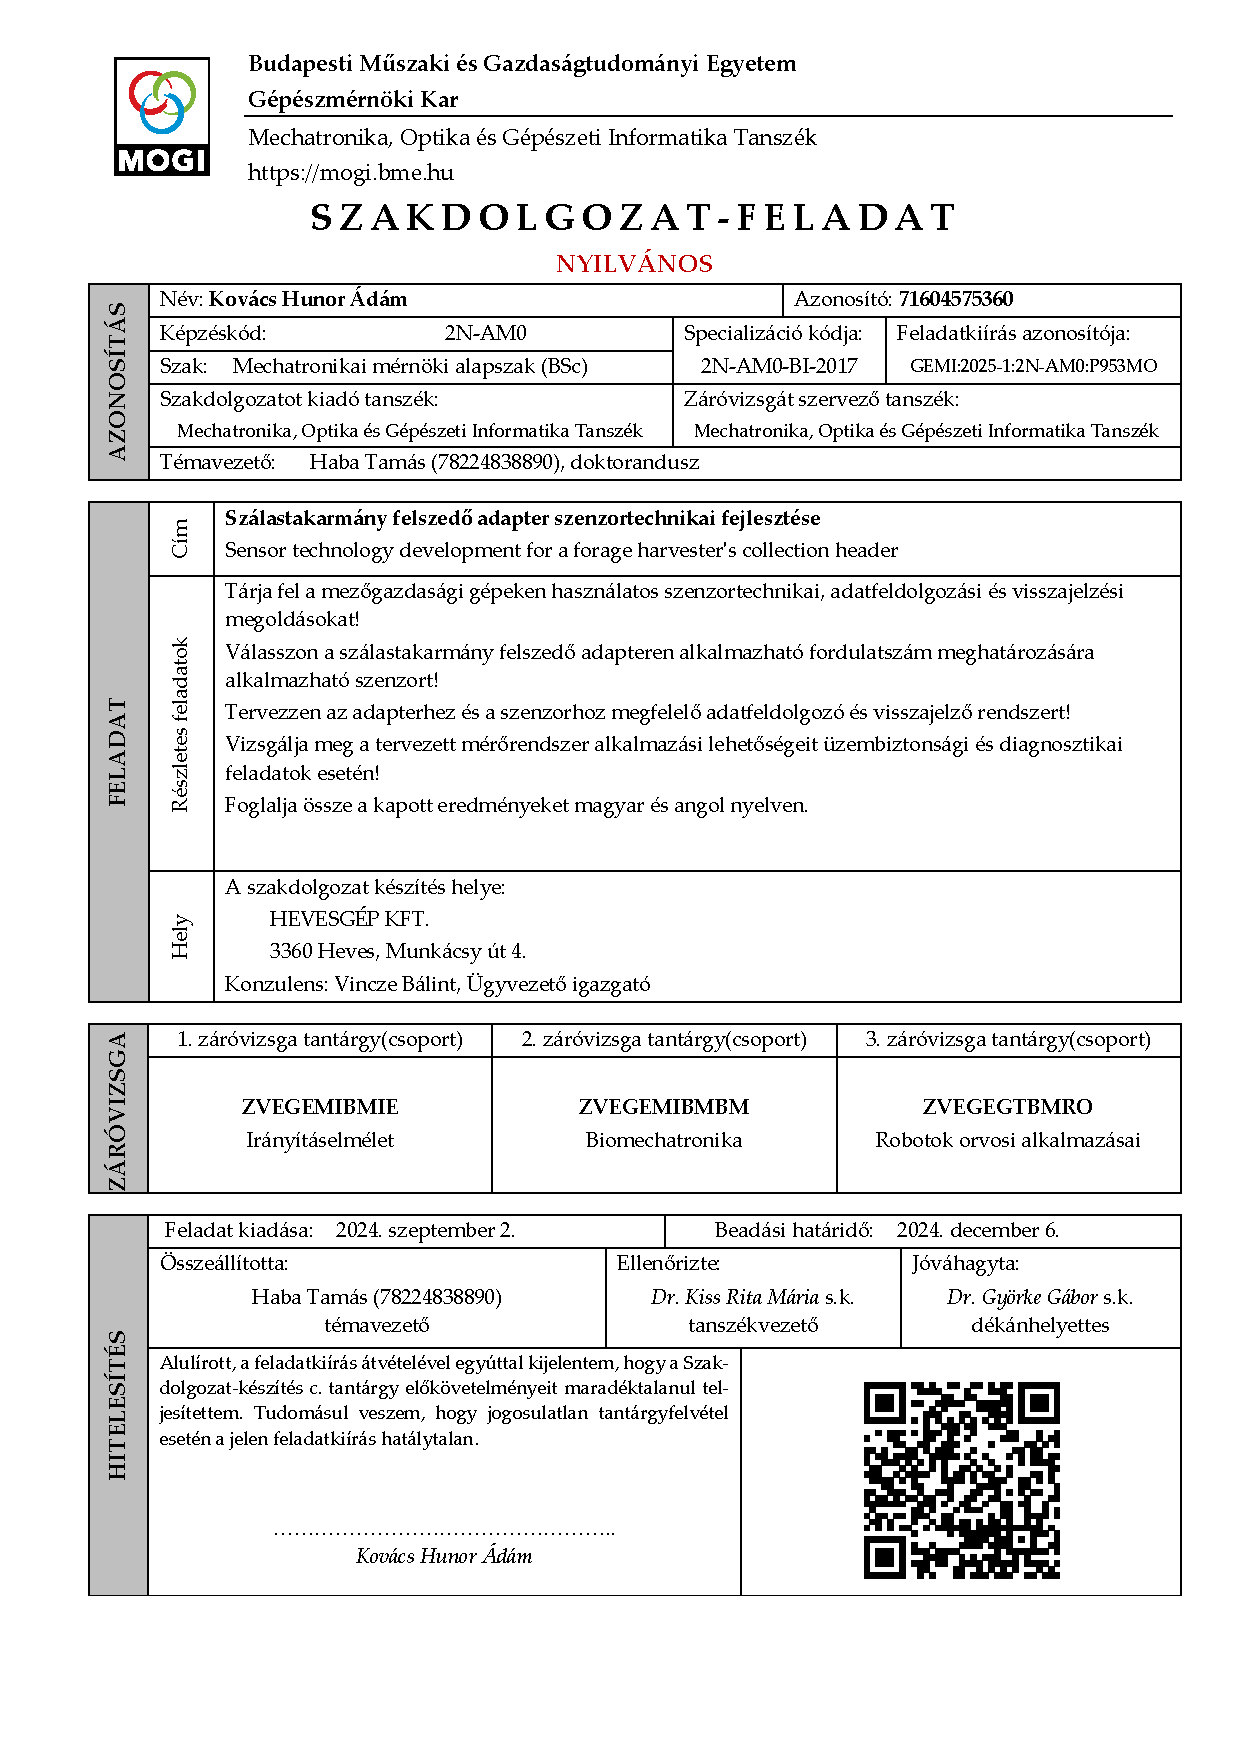
\includegraphics[width=\columnwidth]{MOGI_SZD_P953MO_24o}



% Nyilatkozatok [Declarations]
\selectlanguage{magyar}
\selecthungarian
\pagenumbering{roman}
\setcounter{page}{6}
\cleardoublepage % duplexnél páratlan oldalon legyen
%--------------------------------------------------------------------------------------
% Nyilatkozatok
%--------------------------------------------------------------------------------------
\begin{center}
\section*{NYILATKOZATOK}
\end{center}

\vspace{0.5cm}

\begin{center}
\emph{Beadhatósági nyilatkozat}
\end{center}
A jelen \MakeLowercase{\gpkmunkatipusHU} az üzem/intézmény által elvárt szakmai színvonalnak mind tartalmilag, mind formailag megfelel, beadható.

\begin{flushleft}
Kelt,
\end{flushleft}

\begin{flushright}
 \makebox[7cm][l]{Az üzem részéről:}\\
 \vspace{0.5cm}
 \makebox[7cm]{\rule{6cm}{.4pt}}\\
 \makebox[7cm]{\emph{üzemi konzulens}}
\end{flushright}
\vspace{0.6cm}

%--------------------------------------------------------------------------------------

\begin{center}
\emph{Elfogadási nyilatkozat}
\end{center}
Ezen \MakeLowercase{\gpkmunkatipusHU} a Budapesti Műszaki és Gazdaságtudományi Egyetem Gépészmérnöki Kara által a Diplomatervezési és Szakdolgozat feladatokra előírt valamennyi tartalmi és formai követelménynek, továbbá a feladatkiírásban előírtaknak maradéktalanul eleget tesz. E \MakeLowercase{\gpkmunkatipustHU} a nyilvános bírálatra és nyilvános előadásra alkalmasnak tartom.

\begin{flushleft}
A beadás időpontja:
\end{flushleft}

\begin{flushright}
 \makebox[7cm]{\rule{6cm}{.4pt}}\\
 \makebox[7cm]{\emph{témavezető}}
\end{flushright}
\vspace{0.6cm}

%--------------------------------------------------------------------------------------

\begin{center}
\emph{Nyilatkozat az önálló munkáról}
\end{center}
Alulírott,  \emph{\authorFamilyName{} \authorGivenName} (\neptun), a Budapesti Műszaki és Gazdaságtudományi Egyetem hallgatója, büntetőjogi és fegyelmi felelősségem tudatában kijelentem és sajátkezű aláírásommal igazolom, hogy ezt a \MakeLowercase{\gpkmunkatipustHU} meg nem engedett segítség nélkül, saját magam készítettem, és dolgozatomban csak a megadott forrásokat használtam fel. Minden olyan részt, melyet szó szerint vagy azonos értelemben, de átfogalmazva más forrásból átvettem, egyértelműen, a hatályos előírásoknak megfelelően, a forrás megadásával megjelöltem.

\begin{flushleft}
Budapest, \today
\end{flushleft}

\begin{flushright}
 \makebox[7cm]{\rule{6cm}{.4pt}}\\
 \makebox[7cm]{\emph{hallgató}}
\end{flushright}


\vfill
\clearpage

\selectthesislanguage

\newcounter{romanPage}
\setcounter{romanPage}{\value{page}}
\stepcounter{romanPage}


\selectthesislanguage
% Tartalomjegyzék [Table of Contents]
\setcounter{tocdepth}{3}  % Tartalomjegyzék mélysége [ToC depth]
\tableofcontents\vfill


% Ábrák és táblázatok jegyzéke [List of Figures, Tables]
%TODO Kommenteld ki, ha használni szeretnéd. [Uncomment to use]
%\listoffigures\addcontentsline{toc}{chapter}{\listfigurename}   % Ábrák jegyzéke - opcionális
%\listoftables\addcontentsline{toc}{chapter}{\listtablename}     % Táblázatok jegyzéke - opcionális


% Előszó [Preface]
%----------------------------------------------------------------------------
\chapter*{\eloszo}\addcontentsline{toc}{chapter}{\eloszo}
%----------------------------------------------------------------------------

\begin{center}
    $\thicksim \; \thicksim \; \thicksim$
\end{center}


\subsubsection*{Köszönetnyilvánítás}
\emph{A köszönetnyilvánítás ide írható.} Ez a sablon a Villamosmérnöki és Informatikai Kar Méréstechnika és Információs Rendszerek Tanszék szakdolgozat és diplomaterv sablonja alapján készült. Köszönöm készítőinek és karbantartóinak a munkájukat.


\vspace{0.5cm}

\begin{flushleft}
{Budapest, \today}
\end{flushleft}

\begin{flushright}
\emph{\authorName}
\end{flushright}

\vfill



% Jelölések jegyzéke [Table of Symbols]
%\newcommand{\tss}{\textsuperscript}     % tss = felső index
%%----------------------------------------------------------------------------
%\chapter*{\jelolesek}\addcontentsline{toc}{chapter}{\jelolesek}
%%----------------------------------------------------------------------------
%
%%A táblázatban a többször előforduló jelölések magyar és angol nyelvű elnevezése, 
%%valamint a fizikai mennyiségek esetén annak mértékegysége található. Az egyes 
%%mennyiségek jelölése – ahol lehetséges – megegyezik hazai és a nemzetközi 
%%szakirodalomban elfogadott jelölésekkel. A ritkán alkalmazott jelölések 
%%magyarázata első előfordulási helyüknél található.
%
%%~~~~~~~~~~~~~~~~~~~~~~~~~~~~~~~~~~~~~~~~~~~~~~~~~~~~~~~~~~~~~~~~~~~~~~~~~~~~~~~~~~~~~
%% A táblázatokat ABC rendben kell feltölteni, először mindig a kisbetűvel
%% kezdve. Ha egyazon betűjelnek több értelmezése is van, akkor mindegyiket kü-
%% lön sorban kell feltüntetni. Konstansok esetén az értéket is a táblázatba
%% kell írni.
%% Dimenzió nélküli mennyiségek mértékegysége 1 és nem: – !
%% A jelölésjegyzékben csak SI vagy SI-n kívüli engedélyezett mértékegységeket
%% szabad feltüntetni. Egy dokumentumon belül az SI és pl. az angolszász
%% mértékrendszer nem keverhető!
%%~~~~~~~~~~~~~~~~~~~~~~~~~~~~~~~~~~~~~~~~~~~~~~~~~~~~~~~~~~~~~~~~~~~~~~~~~~~~~~~~~~~~~
%
%%~~~~~~~~~~~~~~~~~~~~~~~~~~~~~~~~~~~~~~~~~~~~~~~~~~~~~~~~~~~~~~~~~~~~~~~~~~~~~~~~~~~~~
%% A Jelölés oszlop alapvetően kurzív betűváltozattal szedendő, a Mértékegység
%% oszlopot álló betűkkel kell szedni. Felső indexhez használható a \tss{}
%% parancs.
%%~~~~~~~~~~~~~~~~~~~~~~~~~~~~~~~~~~~~~~~~~~~~~~~~~~~~~~~~~~~~~~~~~~~~~~~~~~~~~~~~~~~~~
%
%\def\arraystretch{1.5}%  vertical cell padding
%
%
%%\subsubsection*{Latin betűk}
%%\begin{center}
%%    \begin{tabular}{lp{10cm}l}
%%        \hline
%%        Jelölés & Megnevezés, megjegyzés, érték & Mértékegység \\ 
%%        \hline
%%        $g$     & gravitációs gyorsulás (9.81)  & m/s\tss{2}     \\
%%        $p$     & nyomás                        & bar           \\
%%        $s$     & fajlagos entrópia             & J/(kg$\cdot$K)\\
%%        \hline
%%    \end{tabular}    
%%\end{center}
%%
%%
%%
%%\subsubsection*{Görög betűk}
%%\begin{center}
%%    \begin{tabular}{lp{10cm}l}
%%        \hline
%%        Jelölés & Megnevezés, megjegyzés, érték & Mértékegység \\ 
%%        \hline
%%        $\eta$  & hatásfok                      & 1             \\      
%%        $\rho$  & sűrűség                       & kg/m\tss{3}    \\
%%        \hline
%%    \end{tabular}
%%\end{center}
%%
%%
%%
%%\subsubsection*{Indexek, kitevők}
%%\begin{center}
%%    \begin{tabular}{lp{12.8cm}}
%%        \hline
%%        Jelölés & Megnevezés, értelmezés\\ 
%%        \hline
%%        $i$     & általános futóindex (egész szám)  \\
%%        nom     & névleges (nominális) érték        \\
%%        opt     & legkedvezőbb (optimális) érték    \\
%%        \hline
%%    \end{tabular}    
%%\end{center}
%%
%
%\def\arraystretch{1}%  vertical cell padding



% Főszöveg [The main part of the thesis]
\cleardoublepage
\pagenumbering{arabic}
%TODO Importáld a saját fejezeteidet [Import your own content]
%----------------------------------------------------------------------------
\chapter{\bevezetes}
%----------------------------------------------------------------------------

A mezőgazdasági fejlesztésre napjainkban nagyobb szükség van mint valaha, hiszen a növekedő népesség ellátásához, -- a mezőgazdasági területek növekedése nélkül -- intenzívebb és produktívabb termelés szükséges. Az előrejelzések szerint több évtizedig a föld népessége növekedni fog \cite{Lutz2010}, ezen felül a termőföld véges, a mezőgazdasági területek növelése és a korlátlan erdőirtás sem fenntartható \cite{Lawrence2014}. Így a már mezőgazdasági termelésre alkalmazott területek termelékenységének növelése elengedhetetlen. Ehhez a sok tényezős folyamathoz a gépgyártók és mérnökök a technológiai fejlesztés és integráció megvalósításával tudnak hozzájárulni.
Ehhez jelen szakdolgozat célja a mezőgazdasági gépek biztonságát és akadálymentes működését fejleszteni, egy szabályozási rendszer fedélzeti integrálásával. Ezt a működési állapot visszajelzésével, a veszélyes folyamatok megelőzésével igyekszik megvalósítani. A dolgozat ezen rendszer kidolgozását, megtervezését, egyes eszközeinek kiválasztását és megfontolását tárgyalja. 

%----------------------------------------------------------------------------
\section{Feladat bemutatása}
%----------------------------------------------------------------------------

A szakdolgozatom a szálastakarmány felszedő adapter szenzortechnikai fejlesztése címet kapta. A szálastakarmány felszedő adapter a mezőgazdaságban alkalmazott szerkezet, amely a silózoknak hajtja végre a szálastakarmány összegyűjtését. A silózók olyan mezőgazdasági gépek, amelyek a szálastakarmány (pl.: lucerna, széna) begyűjtését, összevágását és rövidre darabolását ("szecskázását") végzik, mely állat tápként lesz felhasználva. Az adapter a silózóhoz van csatlakoztatva, ezáltal a működtetést a silózó végzi. Innen érkezik az irányító jel, az elektromos feszültség, a hidraulikus energia és a forgatónyomaték. Az felszedőn több tengely is található, a legfontosabb a felszedő, melyen fogakkal történik a szálastakarmány gyűjtése, felette egy csiga helyezkedik el, mely az adapter szélességében tereli a takarmányt a középtengely felé, ahol is a begyüjtés történik. A csigánál található tengelyen helyezkedik el egy nyomatékhatároló. A nyomatékhatároló feladata, hogy a túlzott terheléstől megvédje a felszedő adaptert, így ha túl nagy nyomaték érkezik a silózó felől, a nyomatékhatároló szétkapcsol és a felszedő roncsolódása elkerülhető. A nyomatékhatároló szétkapcsolások a benne található tárcsák tapadási súrlódása megszűnik, így elkezdenek csúszni egymáson, amely a tárcsák felületének súrládásához, hosszabb idő alatt roncsolódásához vezet. A nyomatékhatárolók védelme érdekében van szükség egy visszajelző rendszerre, amely a nagy terhelés esetén jelzi az irányítóknak, hogy a nyomatékhatároló megcsúszott.
Az én feladatom ezt a rendszert megtervezni, amely a tengelyek fordulatszámának figyelésével érzékelni tudja ha azok eltérnek a beérkező fordulatszámtól, majd a különbség fennmaradásával egy visszajelzést adjon a silózóban tartózkodó irányítónak. A visszajelzés történhet fény, hang vagy mindkettő formájában, a jelzőegységek lehetnek az adapter látható felületein, vagy akár az irányító fülkében is. Abban az esetben ha a fülkében egy kijelző elhelyezése és azzal való kommunikáció megoldható, a fordulatszámok aktuális értékei is megjelenítésre kerülhetnek.

%----------------------------------------------------------------------------
\section{Célkitűzések}
%----------------------------------------------------------------------------

A dolgozat célja, hogy bemutassa egy mezőgazdasági környezetben való rendszer kialakításának megfontolásait, valamint a tervezési folyamat megvalósítását. Ezen felül az elvárásoknak megfelelő rendszerre való javaslatot tegyen, amely egy termékként alkalmazhatóvá váljék a gyakorlatban is.
A feladat során több olyan irányadó cél, elv mentén történt a tervezés, amely vagy felhasználói, környezeti igényeket elégít ki, vagy a fenntarthatóság, az életciklus növelését segíti.
\begin{enumerate}[I.]
	\item Környezettel, szennyeződésekkel való ellenálló képesség. A felszedő adapteren a két fő szennyező a por és az olaj, így olyan rendszert kell kialakítani, amely vagy szigetelve van kellő mértékben, vagy a szennyeződések nem károsítják a működését. Ez megköveteli az eszközök burkolatban, házban történő tárolását, a csatlakozók kellő szigetelését, illetve por- és olajmentes, vízálló eszközök használatát.
	\item Modularitás, cserélhetőség. A jelen kori gazdák egyik panasza a mezőgazdasági gépgyártók felé, a szerelhetőség jogának ("Right to repair") figyelmen kívül hagyása. Ez a gépek szétszedhetőségét, a felhasználó általi javítási lehetőségének csökkenését jelenti, ezáltal a gyártó szakszervizeiben való költséges, idő- és szállításigényes javításra kötelezi a gazdákat. A cél egy olyan rendszer kialakítása, amelynek minden alkatrésze cserélhető és hozzáférhető, így bármelyik elem meghibásodása során csak az szorul cserére. Ez a szenzorok csatlakozós, nem kábellel egybeépített változatában, a moduláris, egyszerűen szétköthető szabályozó eszközben, valamint, a vízálló csatlakozók szétszedhetőségében nyilvánul meg.
	\item Támogató tervezés csökkentése. A projekt tekintetében egyszerűségre, a mechanikai tervezés csökkentésére törekvés jellemző, a mechatronikai, rendszer tervezésének előnyben részesítése, valamint a felszedő adapter bonyolításának elkerülése végett. Ez az eszközök a meglévő geometriába való integrálásában, az adapter alkatrészeinek direkt mérésében, és a külön szigetelési és burkolási feladatok csökkentésében látható.
	\item Biztonság. A biztonságosság mind a rendszer kitartó működésére, mind a környezetének, üzemeltetőinek megóvására vonatkozik. A projekt során az elektromos berendezések szigetelésére és elzárására, valamint az eszközök külső hatásoktól védésére is hangsúly lett fektetve.
\end{enumerate}

%----------------------------------------------------------------------------
\section{Áttekintés}
%----------------------------------------------------------------------------

A rendszernek 4 alapvető része van: érzékelés (szenzorok), szabályozás, visszajelzés és kommunikáció.
Az érzékelés esetében bemutatásra kerül a különböző fordulatszám mérő mechanizmusok közötti különbség, az egyes mechanizmusok előnyei és hátrányai, valamint ezek alapján a célnak megfelelőek is kiderülnek. A szenzorok megvalósítása is tárgyalva lesz, a különböző rendszerekben alkalmazott szenzor kivitelezések, szabványok és megoldások. Ezen felül a szenzorok elhelyezkedése, kábelezése, a felszedő adapterre való alkalmazásuk is ábrázolva lesz.
A szabályozás során az ipari eszközök lesznek bemutatva, amelyek a szenzorok adatfeldolgozására képesek, valamint programkódokat, irányítási feladatokat kivitelezni tudnak. Szó kerül a különböző megoldások alkalmazásainak lehetőségéről, egymáshoz képesti összehasonlításuk is megtörténik, az egyes szabályozó eszközökkel járó rendszerbeli változtatás, valamint a rendszer igényei szerinti szabályozó eszköz változása is feltérképezésre kerül. Végül a szabályozás eszközeinek elhelyezése, biztonságtechnikai megfontolásai és időállóságának kialakítása is bemutatásra kerül.
A visszajelzés a rendszer mindennapokban érzékelhető része, ugyanis ez az emberrel való kommunikációjának a platformja. A jelzésnek több módszere áll rendelkezésre, melyek között a rendszer adottságai valamint a felhasználó igényei választanak. Az egyszerű fényjelzések, hangjelzésektől egészen a kijelzőkön megjelenő részletes információkig bemutatásra kerül, melyiknek milyen igényei vannak, illetve melyik praktikus jelen felhasználásunkban.
A kommunikáció fogja össze a projektet, biztosítja az egyes részek közötti információáramlást. A kommunikációs protokollok, metódusok meghatározzák a rendszer többi részének minden elemét, a szenzorok feldolgozásának sebességétől, a szabályozó elem kiválasztásán át, a visszajelzés platformjáig. A rendszerünk egészének tervezése során bemutatásra kerül a kommunikáció módszereinek hangsúlya, lehetőségei, valamint a környezeti hatásokkal szemben való védelem kritikus szerepe is.
      			% Bevezetés
%----------------------------------------------------------------------------
\chapter{Szakirodalmi áttekintés}
\label{sec:Szakirodalom}
%----------------------------------------------------------------------------
\section{Szenzorok fajtái}
%----------------------------------------------------------------------------

\subsection{Mérendő mennyiségek}

A feladatom során, a nyomatékhatároló csúszásának meghatározásához az azt megelőző és azutáni tengelyek fordulatszámának összehasonlítására van szükség. Egy tengely fordulatszámának mérésére több megközelítés is létezik. Mérhetjük közvetlenül a tengely elfordulását, akár egy fordulatszámonként egyszer történő jeladást, vagy érzékelhetünk folyamatos változást a tengely kerületén. A jeleket akár integrálhatjuk gyorsulásmérésből, vagy deriválhatjuk szögelfordulásból, azonban ezeknek a pontossága nem minden esetben megfelelő, valamint a számítási igénye is magasabb az ilyen módon nyert jeleknek.

\subsection{Mérési elvek}

\subsection{Szenzor kialakítások}
%----------------------------------------------------------------------------
\section{Jelek feldolgozásának menete}
%----------------------------------------------------------------------------

%----------------------------------------------------------------------------
\section{Szabályozás módszerei}
%----------------------------------------------------------------------------

%----------------------------------------------------------------------------
\section{Visszajelzés lehetőségei}
%----------------------------------------------------------------------------      % 2. fejezet
%----------------------------------------------------------------------------
\chapter{Szenzorok}
\label{sec:Szenzorok}
%----------------------------------------------------------------------------

%----------------------------------------------------------------------------
\section{Mérendő mennyiségek}
%----------------------------------------------------------------------------

%----------------------------------------------------------------------------
\section{Elhelyezés}
%----------------------------------------------------------------------------

%----------------------------------------------------------------------------
\section{Szennyeződések}
%----------------------------------------------------------------------------

%----------------------------------------------------------------------------
\section{Szervizelhetőség}
%----------------------------------------------------------------------------

%----------------------------------------------------------------------------
\section{Kábelezés}
%----------------------------------------------------------------------------
     				% 3. fejezet
%----------------------------------------------------------------------------
\chapter{Jelek}
\label{sec:Jelek}
%----------------------------------------------------------------------------
\section{Szenzorokból származó jelek}
%----------------------------------------------------------------------------

%----------------------------------------------------------------------------
\section{Jelekből adat}
%----------------------------------------------------------------------------
    					% 4. fejezet
%----------------------------------------------------------------------------
\chapter{Szabályozás}
\label{sec:Szabalyozas}

%----------------------------------------------------------------------------
\section{Szabályozás eszközei}
%----------------------------------------------------------------------------

%----------------------------------------------------------------------------
\section{Adatok összehasonlítása}
%----------------------------------------------------------------------------

%----------------------------------------------------------------------------
\section{Hibatűrő rendszer kialakítása}
%----------------------------------------------------------------------------

%----------------------------------------------------------------------------
\section{Visszajelző mechanizmusok}
%----------------------------------------------------------------------------
					% 5. fejezet
%----------------------------------------------------------------------------
\chapter{Visszajelzés}
\label{sec:Visszajelzes}

%----------------------------------------------------------------------------
\section{Visszajelzés eszközei}
%----------------------------------------------------------------------------

%----------------------------------------------------------------------------
\section{Láthatóság, emberi interface}
%----------------------------------------------------------------------------

%----------------------------------------------------------------------------
\section{Kábelezés}
%----------------------------------------------------------------------------					% 6. fejezet
%----------------------------------------------------------------------------
\chapter{Alkalmazási lehetőségek}
\label{sec:Alkalmazas}

%----------------------------------------------------------------------------
\section{Feladat kivitelezésének lehetőségei}
%----------------------------------------------------------------------------

%----------------------------------------------------------------------------
\section{Üzembiztonsági megoldások}
%----------------------------------------------------------------------------

%----------------------------------------------------------------------------
\section{Diagnosztikai feladatok kivitelezése}
%----------------------------------------------------------------------------					% 7. fejezet
%----------------------------------------------------------------------------
\chapter{\osszefoglalas} % (Eredmények értékelése)
%----------------------------------------------------------------------------

%----------------------------------------------------------------------------
\section{Alkalmazási lehetőségek}

%----------------------------------------------------------------------------
\subsection{Feladat kivitelezésének lehetőségei}
%----------------------------------------------------------------------------

%----------------------------------------------------------------------------
\subsection{Üzembiztonsági megoldások}
%----------------------------------------------------------------------------

%----------------------------------------------------------------------------
\subsection{Diagnosztikai feladatok kivitelezése}
%----------------------------------------------------------------------------

%\section{Eredmények}
%Az összefoglaló értékelés a három oldalt lehetőleg ne haladja meg! 
%Az elvégzett munka és eredményeinek bemutatása egyes szám első személyben fogalmazva.
%
%
%\section{Javaslatok/Következtetések/Tanulságok} % Válassz egyet
%A feladat elkészítése során levont tanulságok összefoglalása. Javaslattétel, 
%továbbfejlesztési lehetősége bemutatása, előretekintés a jövőbe stb.

% Keltezés, aláírás
\vspace{0.5cm}

\begin{flushleft}
{Budapest, \today}
\end{flushleft}

\begin{flushright}
\emph{\authorName}
\end{flushright}

\vfill
           			% Összefoglalás


% Bibliográfia [Bibliography]
\addcontentsline{toc}{chapter}{\bibname}
{
    \footnotesize  % Kisebb betűméret [Smaller font size]
    \bibliography{bib/mybib}
}


% Idegen nyelvű (angol) összefoglaló [Foreign language summary]
%----------------------------------------------------------------------------
\chapter*{\summary}\addcontentsline{toc}{chapter}{\summary}
%----------------------------------------------------------------------------

\selectforeignlanguage % angol (magyar) nyelvi beállítások

Az elvégzett munka rövid, másfél oldalt meg nem haladó, de legalább 2/3 
oldalnyi terjedelmű angol nyelvű összefoglalása.

Angol nyelven készített dolgozat esetén magyar nyelvű összefoglaló kell, ha a
készítő magyar anyanyelvű. Nem angol vagy nem magyar nyelven készített
dolgozat esetén kötelező az angol nyelvű összefoglaló, és ha a készítő magyar
anyanyelvű, akkor a magyar nyelvű is.

\vspace{0.5cm}
\paragraph{Keywords} \emph{\keywords}  % A kulcsszavak a fő tex fájlban vannak definiálva


\selectthesislanguage % térjünk vissza magyar (angol) nyelvre



% Függelék és mellékletek [Appendices]
%\excludeFromLocAndLot % A következő ábrákat és a táblázatokat hagyja ki a jegyzékből
                      % [Exclude following figures and tables from List Of Figures/Tables]

%----------------------------------------------------------------------------
\appendix
%----------------------------------------------------------------------------
\chapter*{\fuggelek}\addcontentsline{toc}{chapter}{\fuggelek}
%----------------------------------------------------------------------------
\setcounter{chapter}{\appendixletter} % F betű
%\setcounter{equation}{0}
\numberwithin{equation}{section}
\numberwithin{figure}{section}
\numberwithin{lstlisting}{section}
%\numberwithin{tabular}{section}


% Ismertető - töröld ki
%----------------------------------------------------------------------------
A függelék a főszöveget kiegészíti további részletezéssel. Ide kerül minden kiegészítő információ, ami nem tartozik szorosan a feladat témájához. A függelék rendszerint nem önálló dokumentum. A főszöveg általában nem hivatkozik rá. Általában saját munka.

A dolgozat opcionális eleme, csak igény esetén kell használni.
%----------------------------------------------------------------------------

%----------------------------------------------------------------------------
\section{A TeXstudio felülete}
%----------------------------------------------------------------------------
\begin{figure}[!ht]
\centering
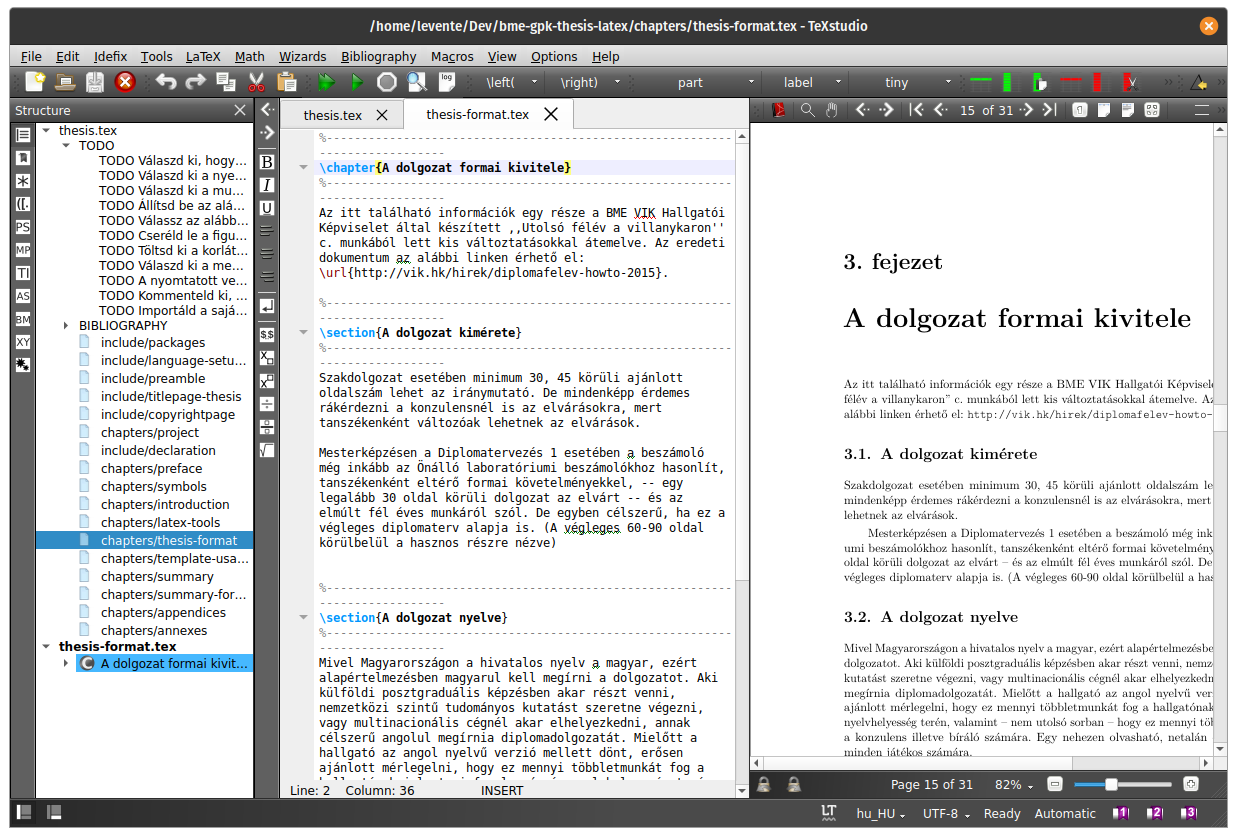
\includegraphics[width=150mm, keepaspectratio]{figures/TeXstudio.png}
\caption{A TeXstudio \LaTeX-szerkesztő.} 
\end{figure}

%----------------------------------------------------------------------------
\clearpage\section{Válasz az ,,Élet, a világmindenség, meg minden'' kérdésére}
%----------------------------------------------------------------------------
A Pitagorasz-tételből levezetve
\begin{align}
c^2=a^2+b^2=42.
\end{align}
A Faraday-indukciós törvényből levezetve
\begin{align}
\rot E=-\frac{dB}{dt}\hspace{1cm}\longrightarrow \hspace{1cm}
U_i=\oint\limits_\mathbf{L}{\mathbf{E}\mathbf{dl}}=-\frac{d}{dt}\int\limits_A{\mathbf{B}\mathbf{da}}=42.
\end{align}
        % Függelék - opcionális
%----------------------------------------------------------------------------
\appendix
%----------------------------------------------------------------------------
\chapter*{\melleklet}\addcontentsline{toc}{chapter}{\melleklet}
%----------------------------------------------------------------------------
\setcounter{chapter}{\annexletter} % M betű
\setcounter{section}{0}
%\setcounter{equation}{0}
\numberwithin{equation}{section}
\numberwithin{figure}{section}
\numberwithin{lstlisting}{section}
%\numberwithin{tabular}{section}

%----------------------------------------------------------------------------
\section{Első melléklet}
%----------------------------------------------------------------------------

A melléklet(ek)ben olyan információkat célszerű elhelyezni, melyek nélkül a főszövegben közöltek nem értelmezhetők, de az ott történő elhelyezésük jelentősen megnövelné a főszöveg terjedelmét. A melléklet rendszerint önállóan is értelmezhető dokumentum. Gyakran nem az író saját munkája. 

A mellékletbe kerülnek például a
\begin{itemize}
  \item terjedelmes, sok adatot tartalmazó táblázatok,
  \item mérési és egyéb jegyzőkönyvek,
  \item levél és faxmásolatok,
  \item szerződésmásolatok,
  \item műszaki rajzok és műszaki leírások,
  \item nagyméretű, ill. összetett kapcsolási vázlatok,
  \item térképek,
  \item fényképek. 
\end{itemize}

A mellékletbe kerülő információ mennyisége esetenként szükségessé teheti több 
melléklet kialakítását. Ebben az esetben célszerű lehet azt például a fenti 
csoportosításban kialakítani, és az egyes mellékleteket folyószámmal ellátni 
(1. Melléklet, 2. Melléklet stb.).
A melléklet tipográfiai kialakítására ugyanazok a szabályok vonatkoznak mint a 
függelékére. 
Minden, a mellékletben található információhordozót (táblázat, ábra, 
fénykép stb.) egyedi számmal és címmel kell ellátni. Ezt az azonosítót kell 
használni a főszövegben az ezekre való hivatkozások során.


%----------------------------------------------------------------------------
\clearpage
\section{Kapcsolási rajzok}
%----------------------------------------------------------------------------

% Képfelirattal ellátott kapcsolási rajzok, táblázatok, fényképek...

\begin{figure}[!ht]
\centering
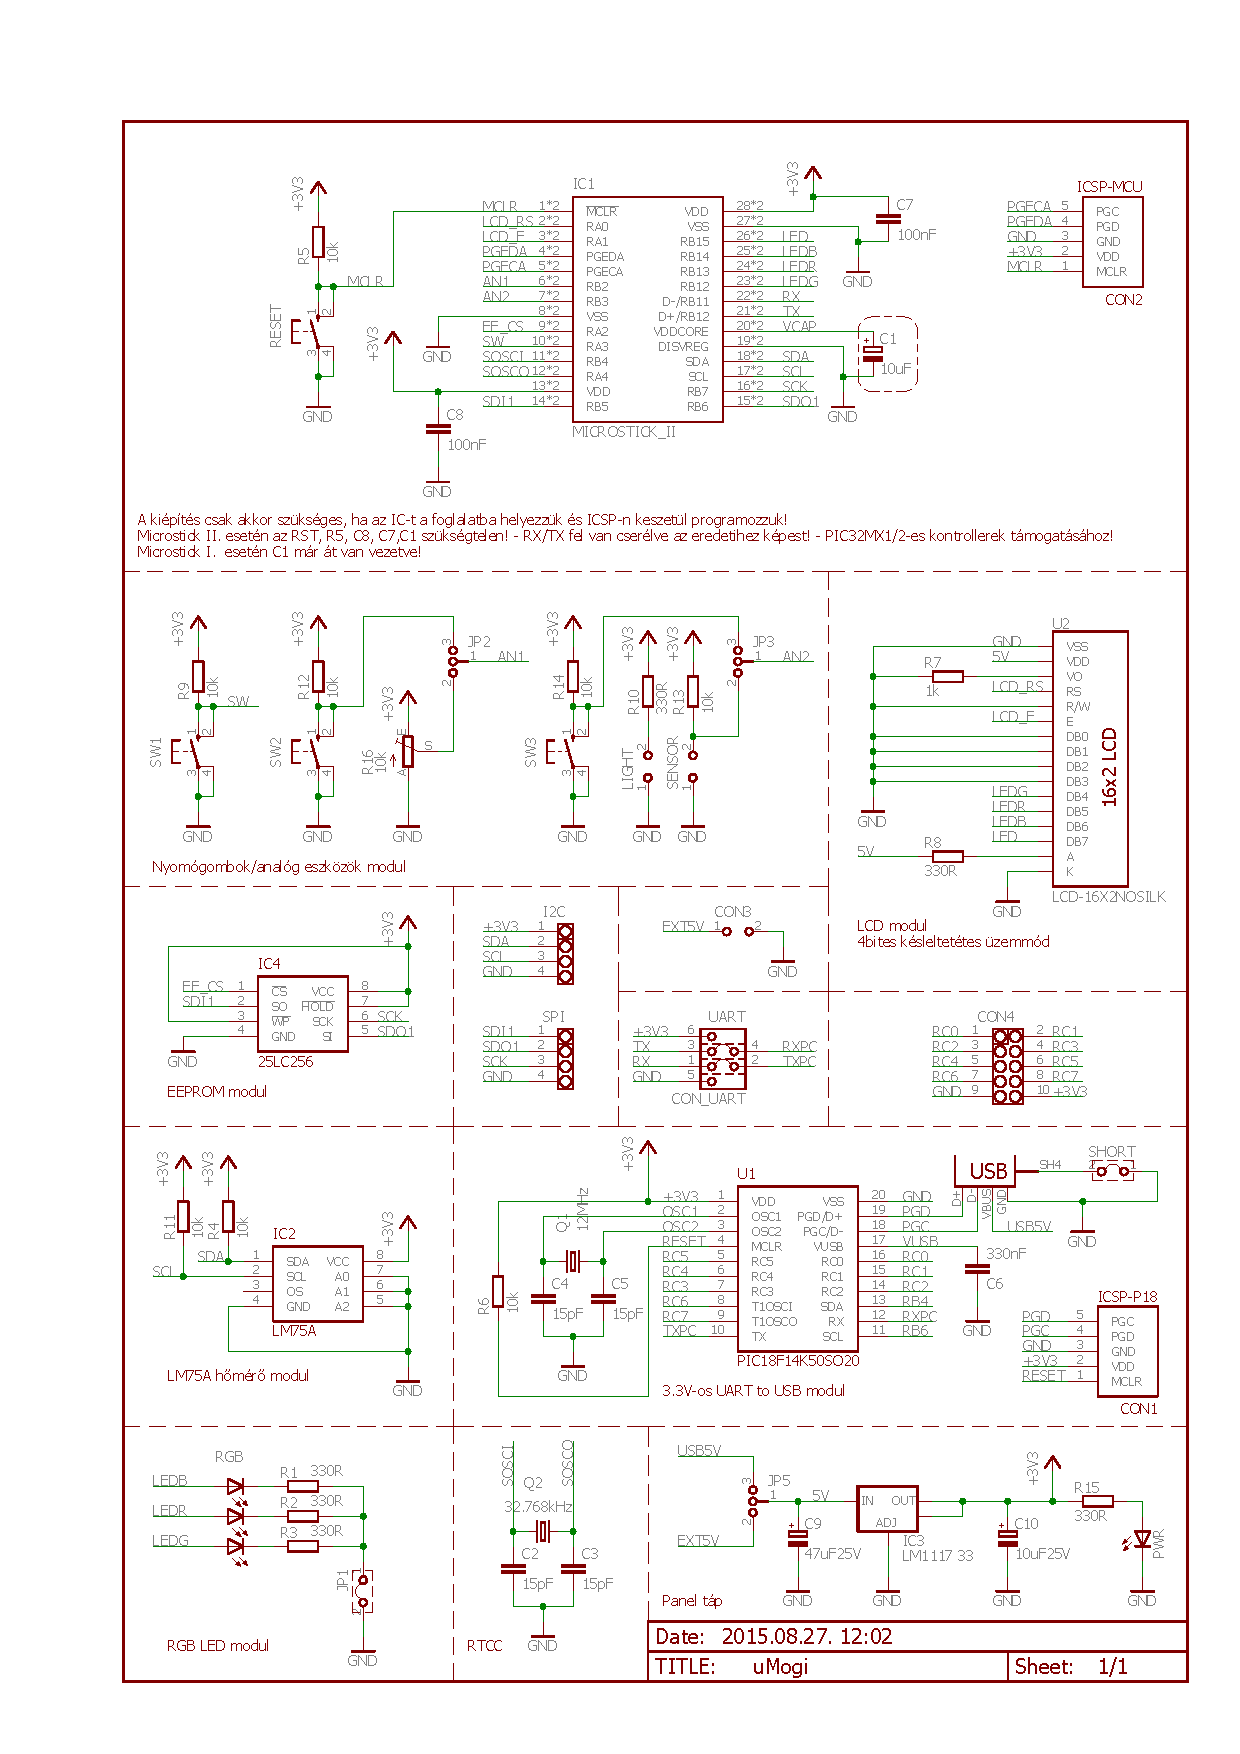
\includegraphics[width=0.9\textwidth, keepaspectratio]{figures/uMogi.pdf}
\caption{A uMogi kapcsolási rajza.} 
\end{figure}
           % Mellékletek

\end{document}
